% For the anonymous EasyChair copy use \documentclass[review]{isi2027}
\documentclass{isi2027}

\begin{document}

\isiTitle{Becoming Informed at Work: Information Behavior of Employees Using Retrieval-Augmented Assistants}

\isiAuthors{Ahmed Ali and Asher Mehfooz}{University of Kotli Azad Jammu and Kashmir, Pakistan\\ rajaahmedalikhan97@gmail.com, info.hasher@gmail.com}

\isiAbstract{Information science studies how people become informed. Workplace retrieval-augmented generation (RAG) assistants now answer operational questions in one fluent utterance while optionally showing snippets. That interface moves the act of becoming informed from a results list a worker can inspect to a generated statement a worker may treat as a source. This paper specifies a model of the informing episode, a six-task battery (factoid, conflict, staleness, absence, informing others, and repair), and a coding book for informed, misinformed, uninformed, overtrust, and repair outcomes. The instrument is validated on an 18-document intranet for a fictional retailer. A transparent BM25 retriever is run on the six task queries. No interviews are invented. The designed situations appear in the retrieved set: a superseded 30-day refund procedure outranks the current 14-day rule; marketing copy promising 30 days outranks the governing procedure on a day-20 case; and a superseded restocking-fee list outranks the current list. Absence is instantiated by a domestic-only warranty record. The contribution is an information-behavior instrument and evidence that lexical RAG can surface the wrong information-as-thing first. A think-aloud protocol is included for later human application.}

\isiKeywords{information behavior; information literacy; retrieval-augmented generation; workplace; becoming informed; source criticism}

\section{Introduction}

The motto of the 19th International Symposium on Information Science (ISI 2027) is Michael Buckland's phrase ``becoming informed and informing others'' \citep{Buckland2017}. In that framing, information science is not primarily the study of storage formats. It is the study of a change of state: a person moves from being less informed to being more informed, and sometimes then informs someone else. For three decades the dominant workplace tools for that move have been search systems and colleagues. A query produces a ranked list. The seeker opens, compares, and rejects documents \citep{Bates1989,Kuhlthau1991,Lewandowski2023}. Colleagues, shared drives, and professional judgement sit beside the list \citep{Bystrom1995,Lloyd2010}.

Retrieval-augmented generation changes the surface of that process. \citet{Lewis2020} introduced RAG as a way to condition a language model on retrieved passages so that generated text depends less on parametric memory alone. In a workplace deployment the worker types a question such as ``what is the refund window for an unopened item?'' and receives a paragraph that sounds like a policy officer. The engineering literature treats failures of that paragraph as hallucination. For information science the sharper question is different. Does the worker become informed, or does the worker stop seeking because the utterance already looks informed?

The question is easy to miss if RAG is evaluated only with answer accuracy. A correct sentence can still leave the worker unable to say which document was used, whether a second policy contradicts the first, or whether the case is simply not in the corpus. A refused answer can leave the worker uninformed and yet better placed to ask a colleague. A fluent wrong answer can produce misinformation that is harder to see than an empty search page. These are informing outcomes, not model scores.

Two workplace facts make the setting distinct. First, the corpus is not Wikipedia. It contains current standard operating procedures, superseded copies, marketing pages, tickets, and memos that do not have the force of a procedure. Second, the worker is often not only becoming informed for themselves. They inform a customer or a supervisor. Buckland's second clause is therefore operational.

This paper does three things. It specifies a conceptual unit of analysis, the informing episode, for workplace RAG. It specifies a reusable task battery and coding book. It validates the instrument on a constructed corpus with a lexical retriever and reports what is actually retrieved. The paper does not report fictional think-aloud participants. Human application is written as a protocol, not as invented results. Three research questions follow:

\begin{enumerate}
  \item How can becoming informed, being misinformed, and remaining uninformed be conceptualised when a RAG assistant mediates a workplace question?
  \item How can conflict, staleness, absence, and informing others be operationalised in a small, inspectable task battery?
  \item When a transparent lexical retriever is run on that battery, do the designed informing situations appear in the retrieved set, and which information-as-thing is ranked first?
\end{enumerate}

Figure~\ref{fig:design} shows the design. Sections~2 and~3 develop theory and related work. Section~4 describes the instrument. Section~5 reports the retrieval validation. Section~6 discusses implications for information literacy next to a RAG box. Section~7 concludes.

\begin{figure}[ht]
  \centering
  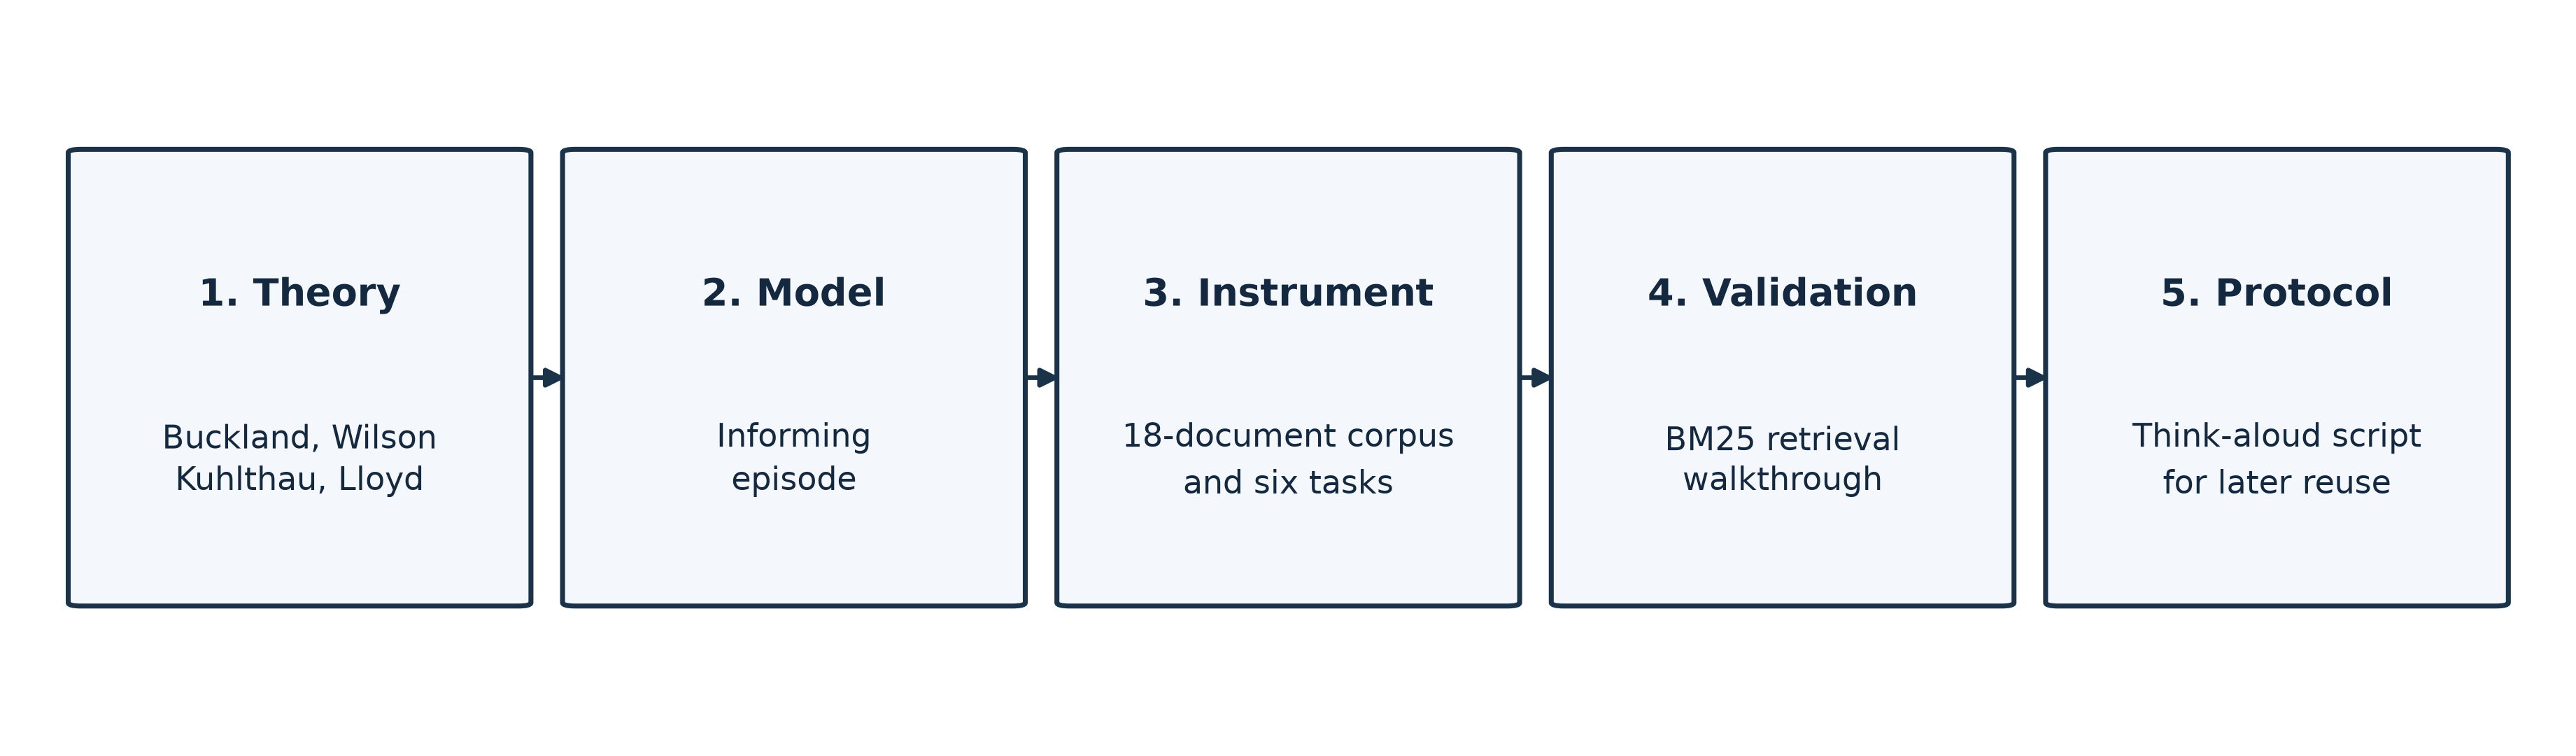
\includegraphics[width=0.98\textwidth]{figures/fig1_research_design.png}
  \caption{Research design. Human think-aloud application is specified for reuse and is not fabricated in this manuscript.}
  \label{fig:design}
\end{figure}

\section{Theoretical Background}

\subsection{Information-as-Thing, Process, and Knowledge}

\citet{Buckland1991} distinguishes three senses of information: as thing, as process, and as knowledge. A procedure file is information-as-thing. The worker's change of state is information-as-process: becoming informed. The rule the worker can later apply is information-as-knowledge. Search engines expose things and leave the process partly visible. The seeker sees that several documents were considered. A generative assistant can collapse thing and process into one utterance. The knowledge state may change without the worker handling a thing. \citet{Buckland2017} later places this process in a social frame: people become informed and they inform others. A workplace RAG box sits on that hinge.

\citet{Wilson1999} models information behavior as nested layers of behavior, seeking, and search, activated by a need and shaped by intervening variables. \citet{Kuhlthau1991,Kuhlthau2004} adds the affective path of the information search process: initiation, selection, exploration, formulation, collection, and presentation, with uncertainty rising before a focus is formed. Both models assume that the seeker remains in contact with identifiable sources long enough to feel uncertainty and to formulate. A RAG answer that arrives in two seconds can skip formulation. The worker may move straight to presentation---telling a customer what ``the system said''---without a collection stage. If that happens, Kuhlthau's zone of intervention moves from the query to the moment after the utterance.

\citet{Savolainen1995} reminds us that people satisfice. In a support desk, ``good enough to close the ticket'' may replace ``informed enough to justify the rule.'' Task complexity research already showed that source use changes with the task \citep{Bystrom1995}. A RAG box is a new source type whose access cost is extremely low. Low cost predicts more use and, without literacy support, more satisficing on the first fluent answer. \citet{Case2016} survey this tradition and still centre seekers who encounter sources as things. The present paper extends that tradition by treating the generated utterance as a new kind of intermediary.

\subsection{Workplace Information Literacy and Source Criticism}

Workplace information literacy is not a checklist of database commands. \citet{Lloyd2010} describes it as a landscape of social, corporeal, and epistemic modalities. People learn what counts as evidence from colleagues and from practice, not only from documents. A RAG assistant that answers from an index of files can look epistemically complete while remaining socially thin. The worker may never learn which colleague owns the exception, or that a file is a draft. Literacy here means treating the assistant as one informing institution among others, asking what is missing, and deciding when to leave the box.

Source criticism in search research has long argued that ranking and interface design shape what people take to be true \citep{Lewandowski2023}. \citet{Bates1989} already described seeking as berrypicking across evolving queries, not as a single perfect question. A citation panel under a RAG answer is not automatically literacy. If workers never open the snippet, the panel is decoration. This paper therefore treats snippet use, version checking, query revision, and escalation to a human as literacy moves.

\subsection{The Informing Episode}

The unit of analysis proposed here is the informing episode (Figure~\ref{fig:episode}). An episode has six observable parts: a workplace task; a query; retrieved information-as-thing; a generated utterance; the worker's uptake; and, where relevant, an act of informing others. Three mutually exclusive outcome states describe the final knowledge position of the episode: informed, misinformed, and uninformed. Overtrust and repair are process codes that may co-occur with an outcome. Informed means the conclusion is licensed by the current governing document and a thing can be named. Misinformed means the conclusion is not licensed. Uninformed means no usable conclusion is reached, including a correct refusal with no next step. Overtrust is acceptance of the utterance without inspecting dated snippets when conflict or staleness is visible. Repair is query revision, snippet comparison, or escalation.

\begin{figure}[ht]
  \centering
  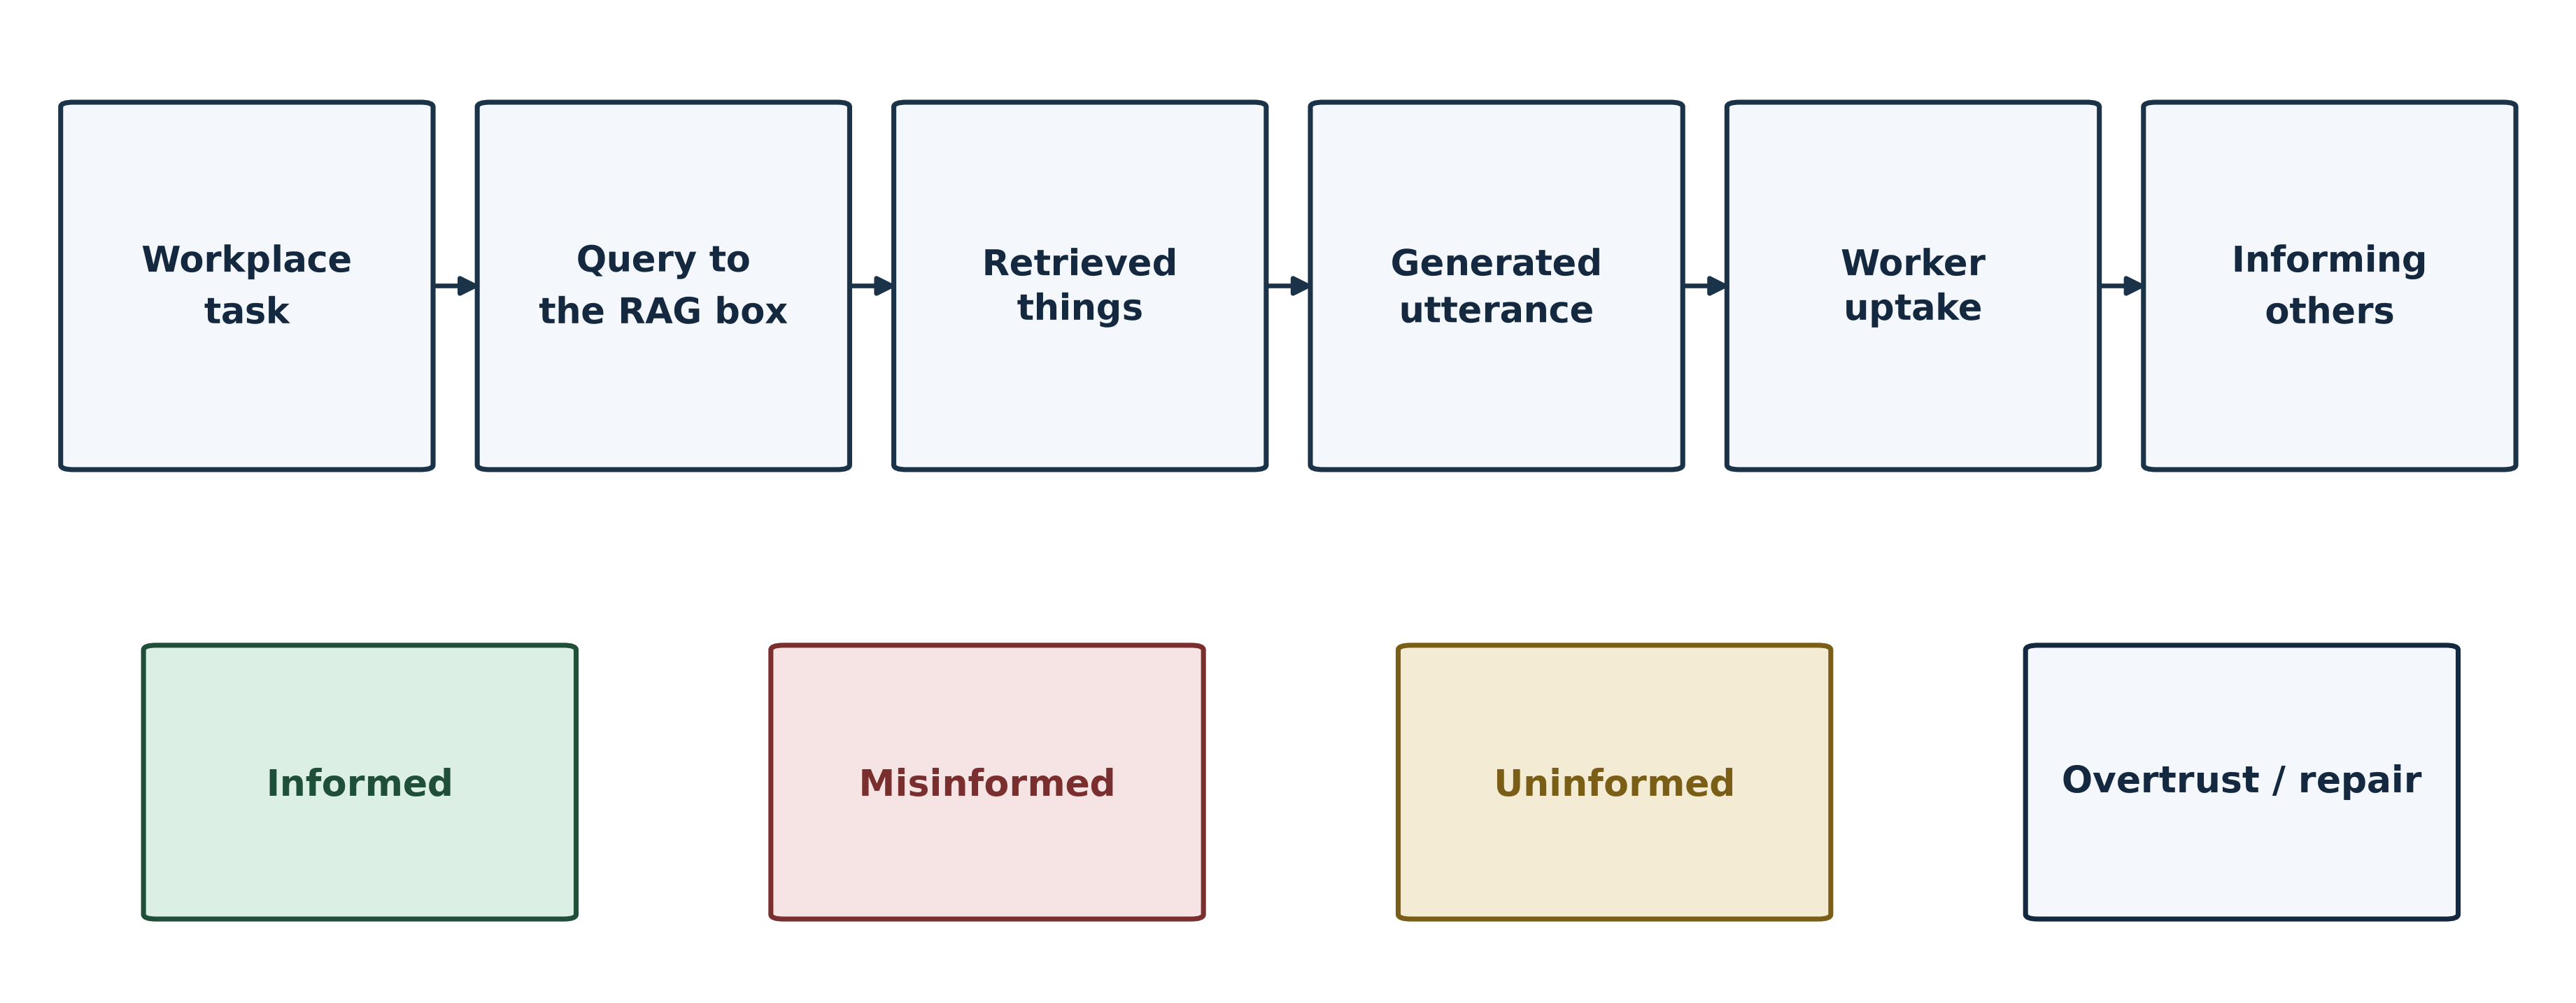
\includegraphics[width=0.98\textwidth]{figures/fig2_informing_episode.png}
  \caption{The informing episode. Outcome states sit under uptake and informing others.}
  \label{fig:episode}
\end{figure}

This model is deliberately smaller than Wilson's nested framework and smaller than Kuhlthau's six stages. It is sized for a RAG turn. The claim is not that those models are obsolete. The claim is that they need an additional object: a generated intermediary that can hide the things it used.

\section{Related Work and Gap}

Workplace information behavior is a large literature. People use colleagues first for many operational questions; documents are used when the task is more complex or more accountable \citep{Bystrom1995,Lloyd2010}. Intranet search studies show that employees struggle with naming, stale pages, and the absence of a single official copy. Those findings predict the failure modes enterprise RAG now meets, but they were produced in a world of links, not generated answers.

Information-behavior research on generative AI is still thin relative to the scale of use. \citet{Gorichanaz2025} analysed 205 public vignettes of ChatGPT use and described six information practices the tool supports: writing, deciding, identifying, ideating, talking, and critiquing. Work appears in that set. The source, however, is an unconstrained chatbot, not a retrieval-grounded workplace assistant, and the method is vignette analysis rather than a controlled task battery. The study is a necessary starting point: it shows that people already treat a generative model as an information source, not only as a writing aid.

The engineering literature on RAG, beginning with \citet{Lewis2020}, measures faithfulness, recall, and generation quality, usually on Wikipedia-scale corpora. Later enterprise benchmarks have shown that those numbers do not transfer cleanly to internal tickets, policies, and acronyms. That is an important retrieval fact. It is not yet an information-behavior fact. Accuracy, latency, and satisfaction can all rise while the worker becomes less able to name a source.

There is therefore a gap between (a)~models of seeking built for search lists and colleagues, (b)~vignette studies of ChatGPT as a general information source, and (c)~RAG papers that never code becoming informed. This paper fills that gap with a model, a task battery, a coding book, and a corpus-level validation. It does not fill it with invented interviews.

\section{Method: Instrument and Validation}

\subsection{Design Choice}

A full think-aloud study with employees is the correct next empirical step and is specified in Section~\ref{sec:protocol}. This manuscript reports the step that can be completed without fabricating people: construction and retrieval validation of the instrument. The design is a conceptual-method study with an empirical corpus walkthrough. That form of theoretical and methodological work is permitted under the ISI full-paper rules. Reviewers should judge the model, the tasks, the coding book, and the retrieval evidence.

\subsection{The Northline Corpus}

A live company corpus cannot be published and would confound the study with unknown missing documents. The field site is a constructed intranet of 18 short English records for a fictional retailer, Northline Parcels. Each record has a title, a date or version, and a function. The set is written so that four informing situations exist as things, not only as story: a current rule, a superseded rule, marketing copy that disagrees with the current rule, and a domain with no document (international warranty). Table~\ref{tab:corpus} lists the records that matter for the six tasks.

\begin{table}[ht]
  \caption{Selected Northline records used to instantiate informing situations.}
  \label{tab:corpus}
  \begin{tabularx}{\textwidth}{@{}lXl@{}}
    \toprule
    Record & Date / status & Informing role \\
    \midrule
    SOP-REFUND-UNOPENED-v3 & 1 March 2026, current & Governing 14-day rule \\
    SOP-REFUND-UNOPENED-v2 & 1 June 2024, superseded & Stale 30-day rule \\
    POLICY-WEB-RETURNS & 12 November 2025, marketing & Conflicting 30-day public copy \\
    PRICE-LIST-2026 / 2024 & 2026 current / 2024 superseded & Stale 8\% versus 15\% fee \\
    SOP-WARRANTY-DOMESTIC & 9 September 2025 & Makes international warranty absent \\
    CHANGELOG-REFUNDS & 1 March 2026 & Repair cue: 30 days withdrawn \\
    \bottomrule
  \end{tabularx}
\end{table}

Other records (damaged-goods procedure, cancel-before-dispatch, privacy, holiday hours, an example ticket, a manager memo) add realistic noise. Noise is required. A corpus that contains only the right procedure would not test informing.

\subsection{Task Battery}

Six tasks force six informing situations (Figure~\ref{fig:tasks}). They are written so that a worker who only reads the top generated sentence can fail in a theoretically interesting way.

\begin{enumerate}
  \item \textbf{T1 Factoid.} What is the refund window for an unopened item? The current procedure says 14 days.
  \item \textbf{T2 Conflict.} A customer wants a refund on day 20. The current procedure says no; the website copy says 30 days. Becoming informed requires seeing the conflict, not averaging the numbers.
  \item \textbf{T3 Stale.} What restocking fee applies to an opened-but-unused return? The current list says 8~percent; the superseded list says 15~percent. The date is the literacy cue.
  \item \textbf{T4 Missing.} How long is the international warranty? No such document exists. Remaining uninformed and escalating is the successful move.
  \item \textbf{T5 Informing others.} Write one sentence to the day-20 customer. Smoothing the conflict away is a distinct failure.
  \item \textbf{T6 Repair.} The assistant said the window is 30 days. Is that still correct? The changelog states that version~3 withdrew the 30-day window.
\end{enumerate}

\begin{figure}[ht]
  \centering
  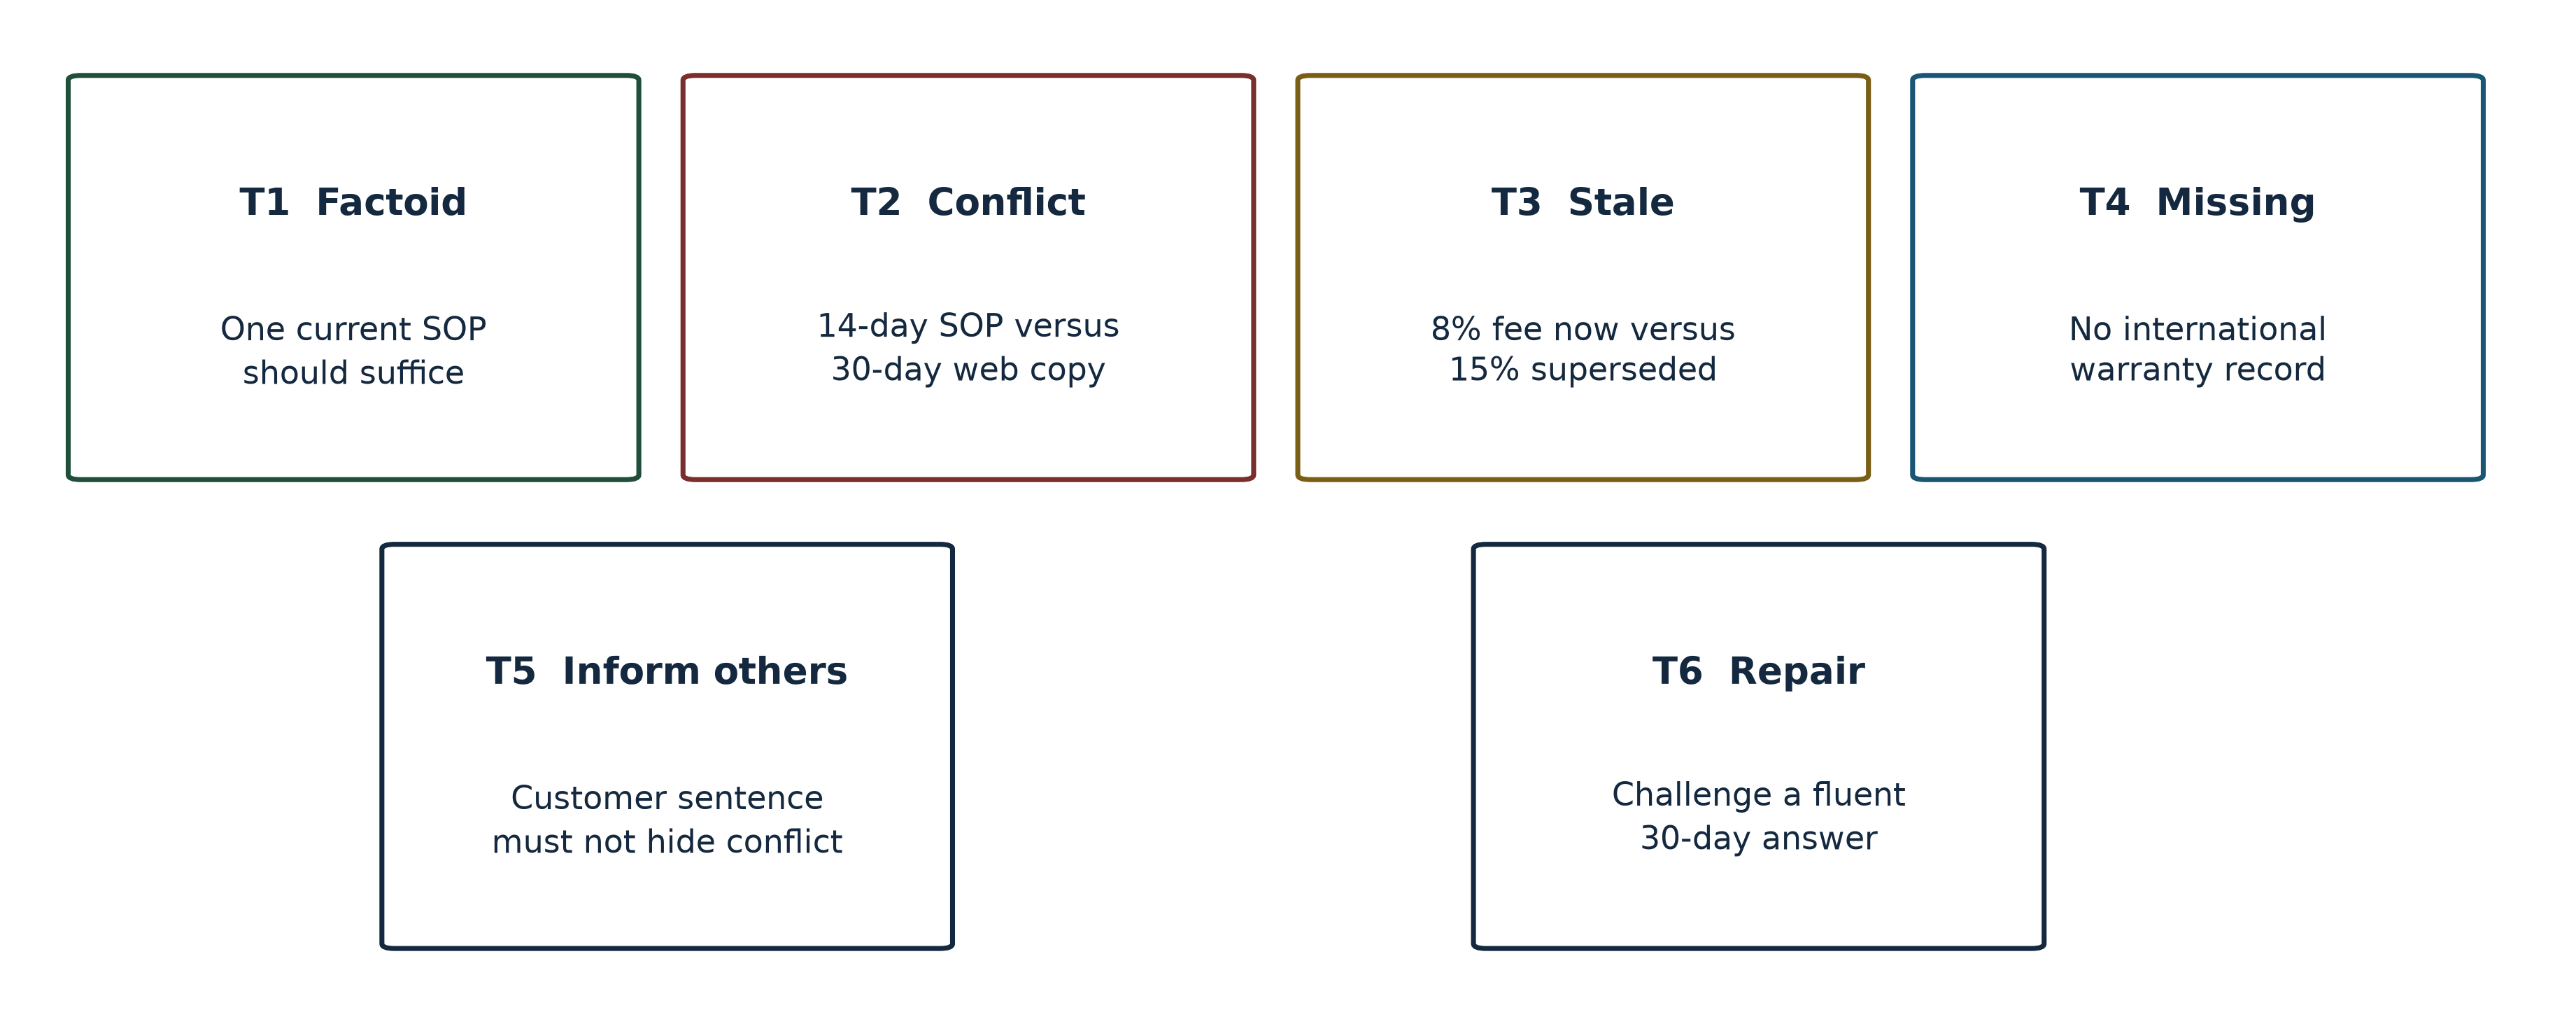
\includegraphics[width=0.98\textwidth]{figures/fig4_task_battery.png}
  \caption{The six-task battery. Each task is an informing situation, not only a query type.}
  \label{fig:tasks}
\end{figure}

\subsection{Retriever}

Validation uses BM25, the standard lexical ranking function \citep{Robertson2009}, with $k_1 = 1.5$ and $b = 0.75$. The retriever is deliberately not a neural embedding model. A lexical ranker is inspectable: a reviewer can see why a superseded procedure that repeats ``unopened,'' ``refund,'' and ``days'' can beat a current procedure. Figure~\ref{fig:arch} places this retriever inside the informing institution: query, things, snippets with dates, optional utterance. In this manuscript the utterance is not sampled from a large language model, because an extra generator would add an uncontrolled source of wording. The retrieval set is the result. That is enough to answer RQ3. A language model can be added later without changing the coding book.

\begin{figure}[ht]
  \centering
  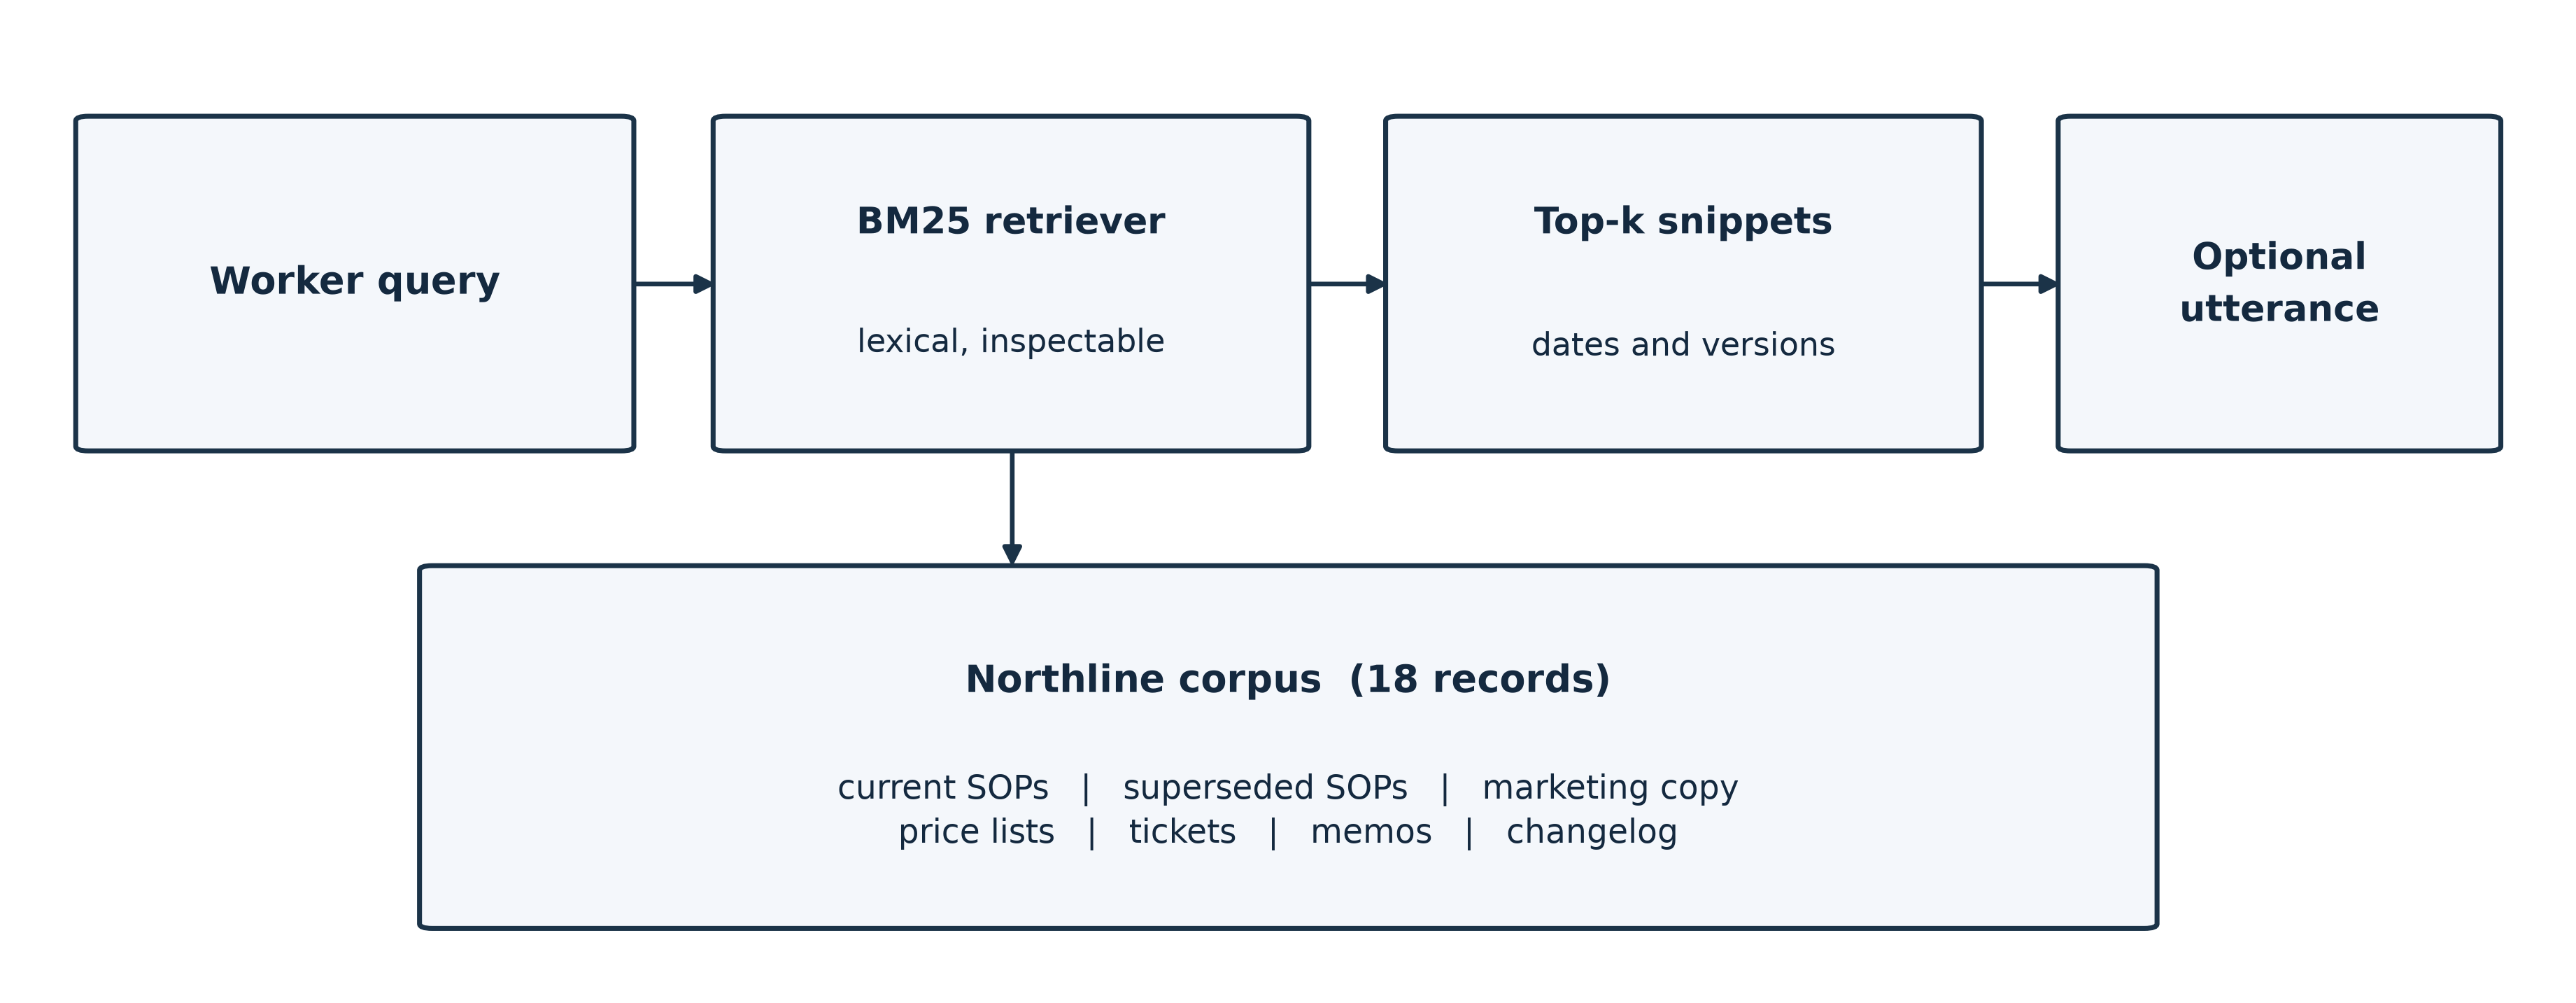
\includegraphics[width=0.98\textwidth]{figures/fig3_rag_architecture.png}
  \caption{RAG treated as an informing institution. The validation in this paper stops at retrieved things plus dates.}
  \label{fig:arch}
\end{figure}

\subsection{Protocol for Later Human Application}
\label{sec:protocol}

For replication with people, the recommended design is a think-aloud laboratory session with 8 to 12 adults who answer operational questions at work, or advanced students with workplace experience used as declared proxies. Participants complete T1 to T6 after a two-minute interface tutorial. Screen and voice are recorded with consent. No real customer data are used. A second coder codes at least 20~percent of episodes. Agreement is reported as percent agreement and Cohen's kappa. That study is not reported here because it has not been run.

\subsection{Coding Book}

\begin{itemize}
  \item \textbf{Informed.} Conclusion licensed by the current governing record; a thing can be named. For T2, informed includes naming the conflict.
  \item \textbf{Misinformed.} Conclusion the corpus does not license.
  \item \textbf{Uninformed.} No usable conclusion, including a correct refusal with no next step.
  \item \textbf{Overtrust.} Acceptance without opening dated snippets when conflict or staleness is on screen.
  \item \textbf{Repair.} Query revision, version check, changelog use, or escalation.
  \item \textbf{Informing-other (T5).} The customer sentence is faithful, smoothed, or fabricated.
\end{itemize}

\section{Results: Retrieval Validation}

Table~\ref{tab:bm25} reports the top three BM25 documents for each task query. Figure~\ref{fig:scores} shows the BM25 score of a pre-specified target document. The targets were chosen before scoring: the current 14-day procedure for T1, T2, and T5; the 2026 price list for T3; the domestic warranty procedure for T4; the changelog for T6.

\begin{table}[ht]
  \caption{Top-three BM25 documents for each task query (higher is better; scores rounded to two decimals).}
  \label{tab:bm25}
  \begin{tabularx}{\textwidth}{@{}lXXX@{}}
    \toprule
    Task & Rank 1 (score) & Rank 2 (score) & Rank 3 (score) \\
    \midrule
    T1 Factoid & SOP-REFUND-v2 (10.48) & SOP-REFUND-v3 (10.05) & POLICY-WEB (4.49) \\
    T2 Conflict & POLICY-WEB (10.99) & SOP-DAMAGED (7.17) & SOP-REFUND-v3 (6.34) \\
    T3 Stale fee & PRICE-2024 (11.91) & PRICE-2026 (10.56) & POLICY-WEB (5.80) \\
    T4 Missing & WARR-DOM (9.66) & POLICY-WEB (3.56) & SOP-REFUND-v3 (2.42) \\
    T5 Inform others & SOP-REFUND-v3 (3.93) & SOP-DAMAGED (3.32) & TICKET-4412 (3.28) \\
    T6 Repair & CHANGELOG (7.78) & SOP-REFUND-v3 (7.15) & HOLIDAY (5.95) \\
    \bottomrule
  \end{tabularx}
\end{table}

{\small\noindent\textit{Note.} SOP-REFUND-v2/v3 = SOP-REFUND-UNOPENED-v2/v3; POLICY-WEB = POLICY-WEB-RETURNS; WARR-DOM = SOP-WARRANTY-DOMESTIC; HOLIDAY = HOLIDAY-HOURS.}

\begin{figure}[ht]
  \centering
  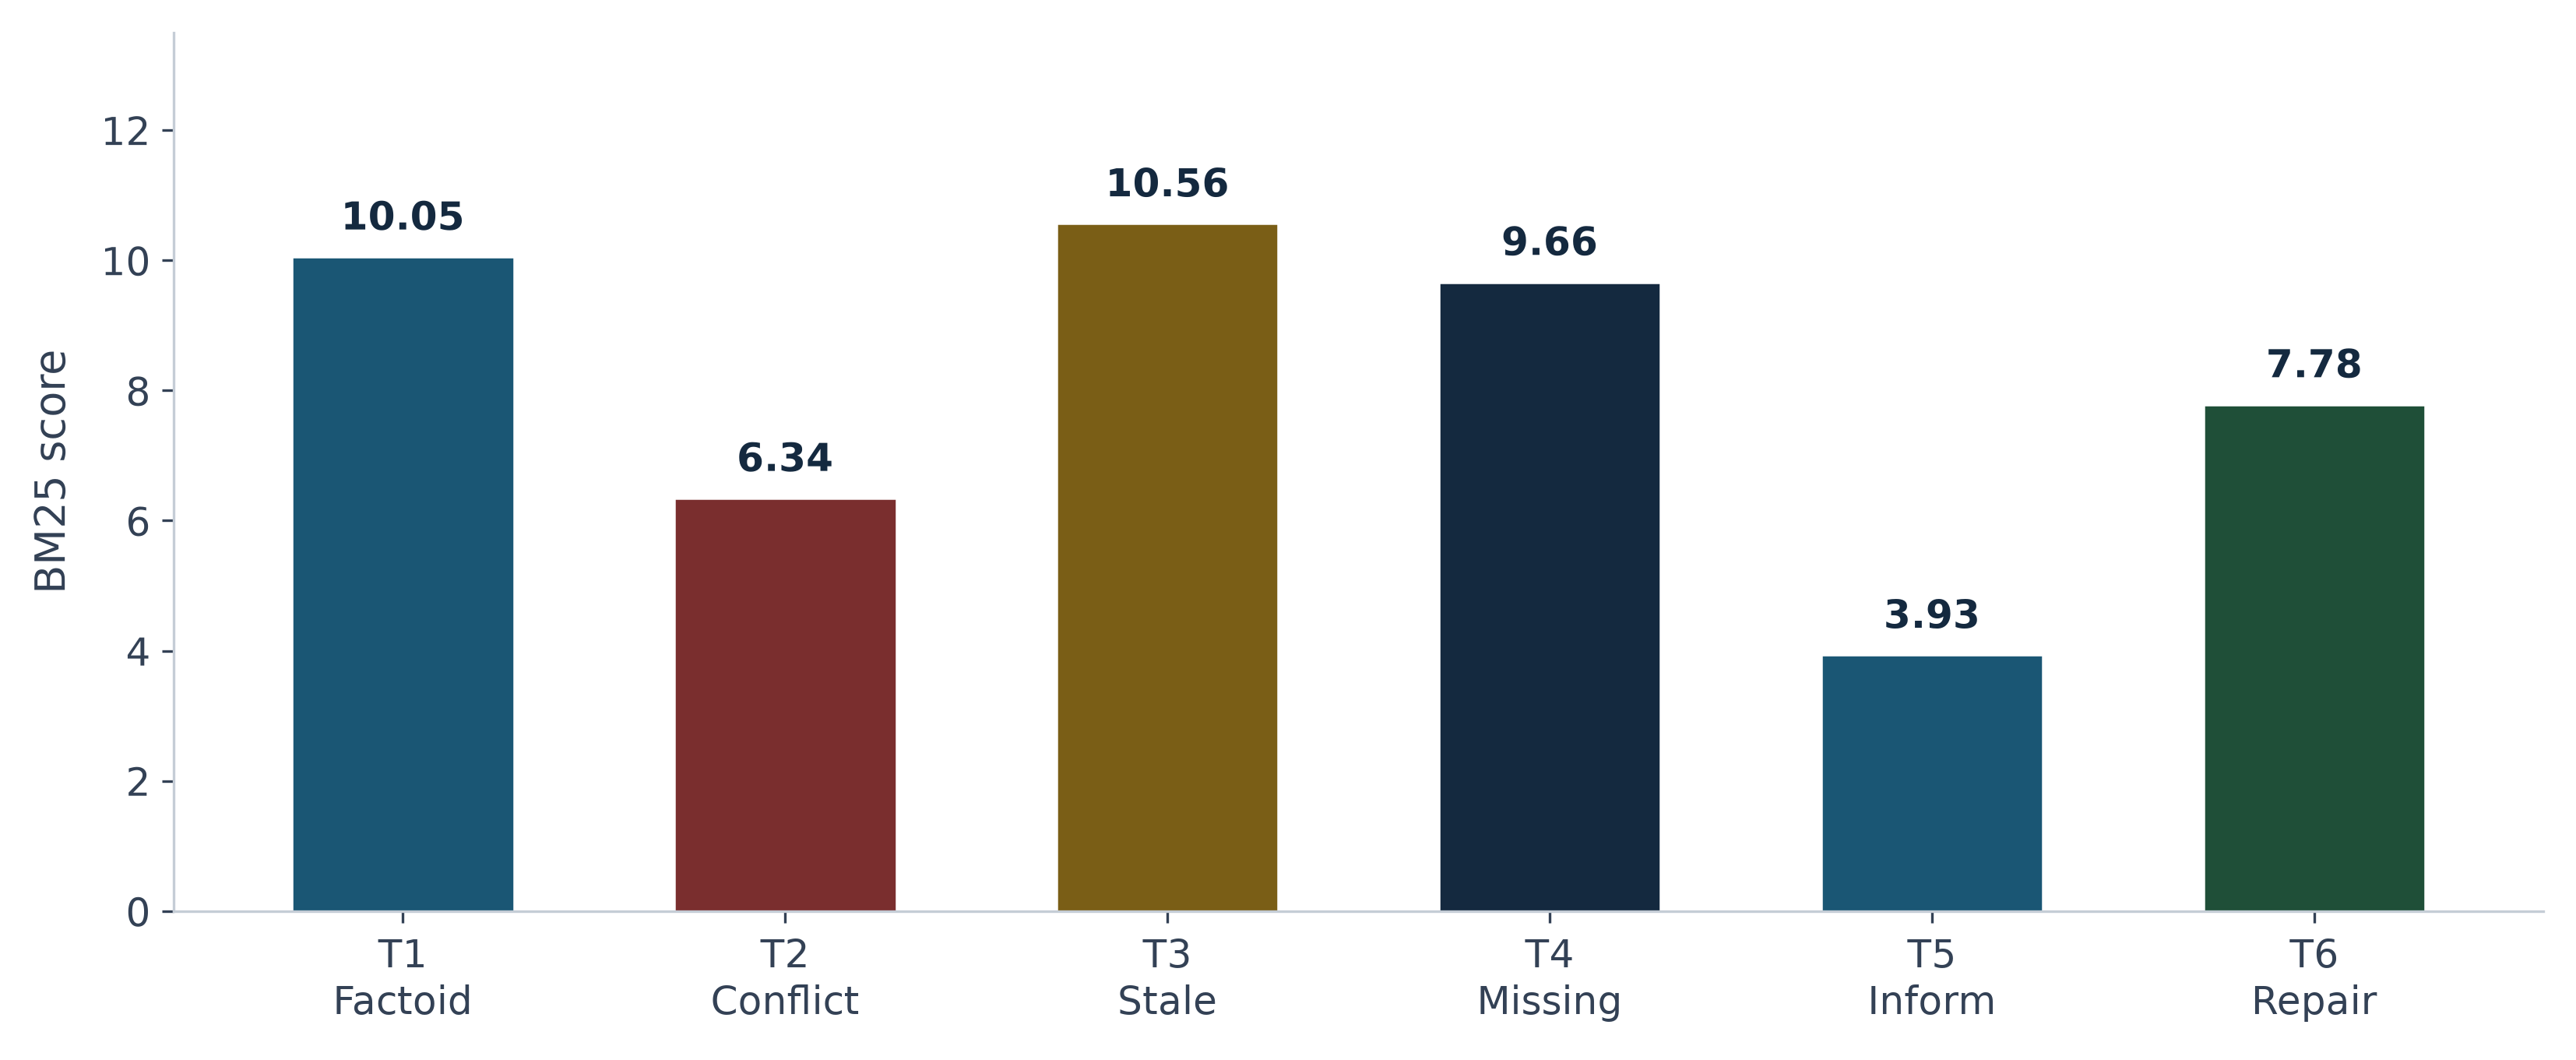
\includegraphics[width=0.98\textwidth]{figures/fig5_retrieval_scores.png}
  \caption{BM25 score of the pre-specified target document. A high score does not mean the target was ranked first.}
  \label{fig:scores}
\end{figure}

\subsection{Factoid and Staleness (T1, T3)}

On T1 the superseded 30-day procedure (v2) scores 10.48 and the current 14-day procedure (v3) scores 10.05. Both are retrieved. The wrong information-as-thing is ranked first. The two texts share the same lexical frame: unopened, refund, packaging, days. BM25 has no notion of ``effective date.'' A worker who trusts rank order, or a generator that conditions only on the first passage, is set up to become misinformed while still ``using retrieval.''

T3 repeats the pattern for a fee rather than a day count. The 2024 price list (15~percent restocking fee) scores 11.91; the 2026 list (8~percent) scores 10.56. Staleness is not a rare edge case in this corpus. It is the default lexical winner when the superseded file is a close paraphrase of the current file. That is a common intranet practice: staff keep the old file ``just in case.''

\subsection{Conflict (T2) and Informing Others (T5)}

On T2 the customer-facing web policy that advertises a 30-day window is ranked first (10.99). The governing 14-day procedure is third (6.34). A damaged-goods procedure sits in between because the query mentions a customer and a refund. The conflict is therefore not only present in the corpus. It is present in the top of the retrieved set, and the public-facing thing outranks the internal governing thing. A generator that summarises the top passage will tell the worker that day~20 is allowed. The worker who then informs the customer (T5) will transmit marketing copy as if it were policy. T5 itself retrieves the current procedure first, which shows that query wording matters: ``write one sentence'' plus ``day-20'' plus ``unopened refund'' is closer to the internal title than ``can we refund.'' Informing others is query-sensitive. That is a result, not a slogan.

\subsection{Absence (T4) and Repair (T6)}

T4 asks for an international warranty. The only warranty record is domestic and explicitly says foreign addresses must be escalated and that no period should be quoted. It is ranked first (9.66). Absence is therefore instantiated as a retrieved refusal instruction, not as an empty index. Remaining uninformed about a number, and escalating, is the informed move. A generator that completes ``12 months'' from the domestic sentence would produce misinformation by over-generalising a real thing.

T6 asks whether a 30-day answer is still correct. The changelog, which states that version~3 withdrew the 30-day window on 1~March 2026, is ranked first (7.78), with the current procedure second. Repair is therefore supported by an information-as-thing that names the change. A literacy interface that never surfaces changelogs hides the repair cue that this corpus actually contains.

\subsection{What the Validation Does and Does Not Show}

The validation shows that RQ2's situations are not fictional labels. They appear in a lexical top-$k$. It shows that rank~1 is often the superseded or public copy, not the governing procedure. It does not show how employees act. It does not measure a language model's wording. It does not claim that dense retrieval would fail in the same way, although nothing in the model requires BM25; a dense index can be swapped without changing the coding book.

\section{Discussion}

\subsection{Ranked Things Are Not Yet Becoming Informed}

The central empirical observation is simple. On the two most ordinary workplace questions---how many days, how large a fee---the first thing retrieved is the old thing. If becoming informed were identical with ``the system retrieved something relevant,'' both T1 and T3 would already look successful. In Buckland's terms they are successful at exposing information-as-thing and unsuccessful at guaranteeing information-as-process. A 30-day procedure that is lexically relevant is still the wrong knowledge. Information science has known this about search result pages for a long time \citep{Lewandowski2023}. RAG makes the problem quieter, because the old thing can be rewritten as a confident new sentence.

Kuhlthau's \citep{Kuhlthau1991} zone of intervention therefore moves. In a search list the intervention is help with formulation while uncertainty is still visible. In a RAG box uncertainty may never appear. The worker is handed presentation without exploration. The implication for information professionals is not only ``add citations.'' It is to restore a collection stage: dates, versions, and a visible second thing when two windows disagree.

\subsection{Conflict Is a Literacy Object}

T2 is the result that belongs at this symposium. Marketing copy outranks the procedure. That is a realistic workplace arrangement: communications teams publish friendlier numbers than operations will honour. A retriever that maximises lexical match to ``refund'' and ``customer'' will prefer the public page. Hybrid search will not dissolve the institutional fact that two things disagree. Lloyd's \citep{Lloyd2010} landscape is useful here. The social modality (what we say on the website) and the epistemic modality (what the desk is allowed to do) are both in the index. Literacy is the capacity to see that they are not the same source type. A coding book that has only ``correct / incorrect answer'' cannot see that. The informed outcome on T2 is naming the conflict.

\subsection{Refusal and Informing Others}

T4 shows that absence can be represented as a document that forbids a number. Remaining uninformed is then a responsible state, not a failed session. Savolainen's \citep{Savolainen1995} satisficing predicts the opposite workplace move: invent a 12-month international warranty because the domestic procedure is nearby. T5 shows why that matters beyond the individual. Once the worker informs a customer, the episode leaves the organisation's internal landscape. A smoothed sentence that hides the 14-versus-30 conflict is an institutional misinforming act. Buckland's motto is then literal.

\subsection{Implications for RAG Design}

Three design implications follow from the retrieval evidence and from the model, without requiring a user sample. First, dates and version status must be first-class snippet fields, not metadata buried in a filename. T1 and T3 are otherwise indistinguishable from success. Second, when two retrieved things disagree on a slot (days, percent, warranty scope), the interface should not average them and should not hide one. That is a literacy intervention in Kuhlthau's sense. Third, changelogs should be retrievable on repair queries. T6 shows that the corpus already contains the repair cue if the system is willing to surface it.

None of these implications is a new neural architecture. They are information-organization decisions \citep{Buckland1991}: which things are marked current, which things are marked public, and whether the process of becoming informed is allowed to see that marking.

\subsection{Limits}

The corpus is fictional and English-only. Eighteen documents are enough to instantiate the situations and small enough to audit by hand; they are not a company. BM25 is one retriever. A dense or hybrid ranker might promote the current procedure more often, or might not; that is an open measurement, not a reason to discard the coding book. No language-model wording is reported, so fluency effects are discussed from theory and from \citet{Gorichanaz2025}, not from this run. No employees were observed. Claims about overtrust remain hypotheses. The paper's results answer RQ3 and support the operationalisation in RQ2. They do not answer how workers behave. Anyone citing this paper as a user study would be mis-citing it.

\section{Conclusion}

Workplace RAG is being built as knowledge management. It is also an informing institution. This paper specified how information science can study that institution without reducing it to retrieval metrics and without inventing participants. The informing episode, the six-task battery, and the coding book turn Buckland's motto into observable moves. The Northline validation shows that those moves are not hypothetical. A current 14-day rule, a superseded 30-day rule, and a 30-day marketing page can sit in one index, and a standard lexical ranker will often put the non-governing thing first. Becoming informed then depends on whether the worker, or the interface, still treats dates and source types as part of the process. That is an information-science problem. The next paper, if it is written honestly, will apply the coding book to recorded workers. This paper stops where the evidence stops.

\section*{Acknowledgements}

\ifisireview Omitted for double-blind review.\else None.\fi

\section*{Appendix A. Think-Aloud Script for Reuse}

Consent. Two-minute tour of snippets and dates. Think aloud. T1 to T6 in fixed order. Exit question: if a customer were on the phone after T2 and after T4, what would you say? Stop recording. Do not help unless the interface breaks.

\section*{Appendix B. Reproducibility}

The 18 corpus files and the BM25 scores used in Table~\ref{tab:bm25} accompany this submission. Rerunning the lexical ranker with $k_1 = 1.5$ and $b = 0.75$ reproduces the table.

%% APA references (verified). natbib authoryear matches the official ISI APA rule.
\begin{thebibliography}{99}

\bibitem[Bates(1989)]{Bates1989}
Bates, M. J. (1989). The design of browsing and berrypicking techniques for the online search interface. \textit{Online Review, 13}(5), 407--424. https://doi.org/10.1108/eb024320

\bibitem[Buckland(1991)]{Buckland1991}
Buckland, M. (1991). Information as thing. \textit{Journal of the American Society for Information Science, 42}(5), 351--360. https://doi.org/10.1002/(SICI)1097-4571(199106)42:5\textless351::AID-ASI5\textgreater3.0.CO;2-3

\bibitem[Buckland(2017)]{Buckland2017}
Buckland, M. (2017). \textit{Information and society}. MIT Press.

\bibitem[Bystr\"{o}m and J\"{a}rvelin(1995)]{Bystrom1995}
Bystr\"{o}m, K., \& J\"{a}rvelin, K. (1995). Task complexity affects information seeking and use. \textit{Information Processing \& Management, 31}(2), 191--213. https://doi.org/10.1016/0306-4573(95)80035-R

\bibitem[Case and Given(2016)]{Case2016}
Case, D. O., \& Given, L. M. (2016). \textit{Looking for information: A survey of research on information seeking, needs, and behavior} (4th ed.). Emerald.

\bibitem[Gorichanaz(2025)]{Gorichanaz2025}
Gorichanaz, T. (2025). Information needs and practices supported by ChatGPT. \textit{Proceedings of the Association for Information Science and Technology, 62}(1), 253--262. https://doi.org/10.1002/pra2.1253

\bibitem[Kuhlthau(1991)]{Kuhlthau1991}
Kuhlthau, C. C. (1991). Inside the search process: Information seeking from the user's perspective. \textit{Journal of the American Society for Information Science, 42}(5), 361--371. https://doi.org/10.1002/(SICI)1097-4571(199106)42:5\textless361::AID-ASI6\textgreater3.0.CO;2-\#

\bibitem[Kuhlthau(2004)]{Kuhlthau2004}
Kuhlthau, C. C. (2004). \textit{Seeking meaning: A process approach to library and information services} (2nd ed.). Libraries Unlimited.

\bibitem[Lewandowski(2023)]{Lewandowski2023}
Lewandowski, D. (2023). \textit{Understanding search engines}. Springer. https://doi.org/10.1007/978-3-031-22789-9

\bibitem[Lewis et~al.(2020)]{Lewis2020}
Lewis, P., Perez, E., Piktus, A., Petroni, F., Karpukhin, V., Goyal, N., K\"{u}ttler, H., Lewis, M., Yih, W., Rockt\"{a}schel, T., Riedel, S., \& Kiela, D. (2020). Retrieval-augmented generation for knowledge-intensive NLP tasks. \textit{Advances in Neural Information Processing Systems, 33}, 9459--9474.

\bibitem[Lloyd(2010)]{Lloyd2010}
Lloyd, A. (2010). \textit{Information literacy landscapes: Information literacy in education, workplace and everyday contexts}. Chandos.

\bibitem[Robertson and Zaragoza(2009)]{Robertson2009}
Robertson, S. E., \& Zaragoza, H. (2009). The probabilistic relevance framework: BM25 and beyond. \textit{Foundations and Trends in Information Retrieval, 3}(4), 333--389. https://doi.org/10.1561/1500000019

\bibitem[Savolainen(1995)]{Savolainen1995}
Savolainen, R. (1995). Everyday life information seeking: Approaching information seeking in the context of ``way of life.'' \textit{Library \& Information Science Research, 17}(3), 259--294. https://doi.org/10.1016/0740-8188(95)90048-9

\bibitem[Wilson(1999)]{Wilson1999}
Wilson, T. D. (1999). Models in information behaviour research. \textit{Journal of Documentation, 55}(3), 249--270. https://doi.org/10.1108/EUM0000000007145
\end{thebibliography}

\end{document}
